\chapter{Experimental Car Platform}

For the purpose of this thesis an experimental car platform was built.
The goal of this project was to evaluate the algorithms described in this thesis not only in simulation but also on a real world robot which is able to reach high speeds. The inspiration comes from the F1/10 Autonomous Racing Competition \cite{f1tenth} and many of the resources and tutorials were used either directly or as an inspiration for assembling and configuring the whole platform.

\section{Chassis}

The base of the experimental vehicle is a commonly available 1:10 scale RC car model with all wheel drive. From the many available models we chose the BEAST BX Buggy RTR 1/10 Brushed \cite{beast} because of its good performance, reasonable price, and good availability of spare parts.

\begin{figure}
    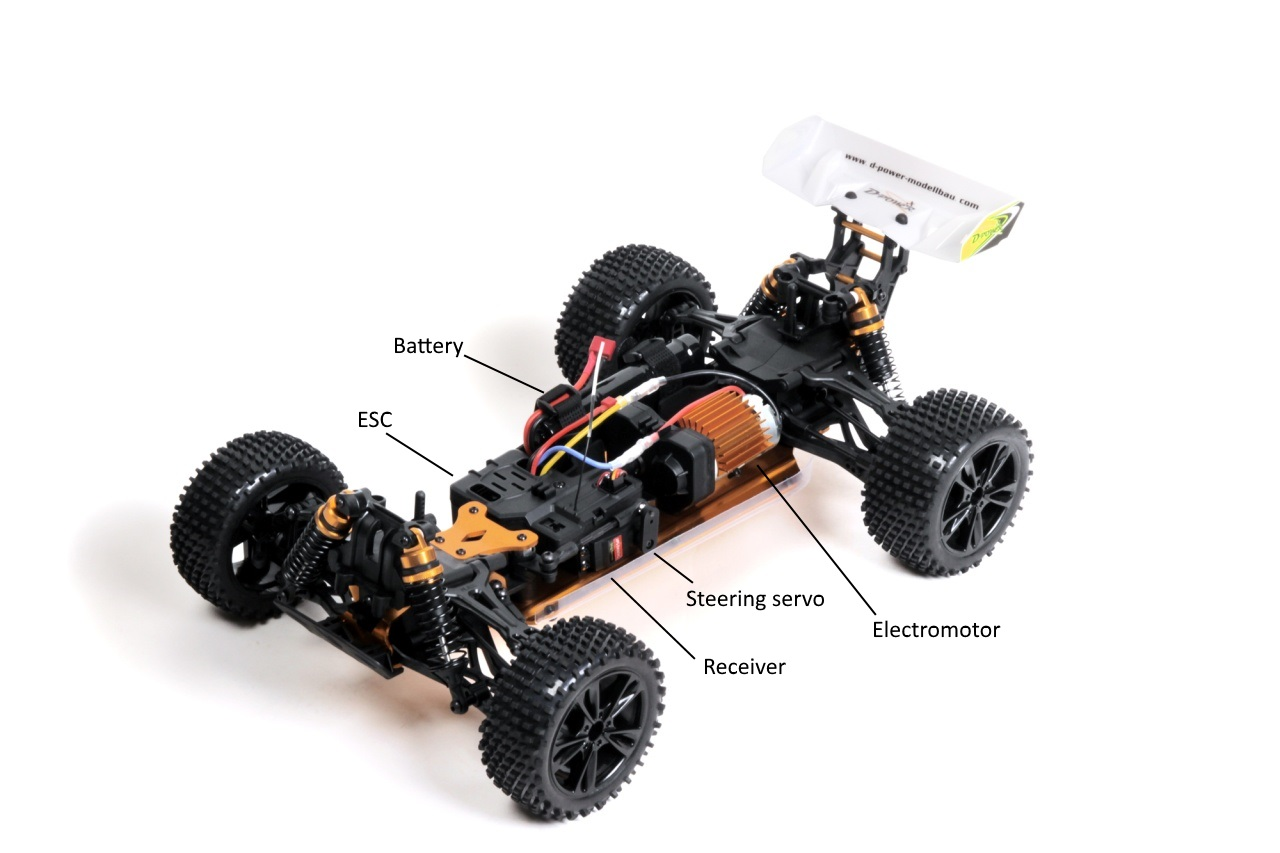
\includegraphics[width=\textwidth]{../img/beast-without-cover.jpg}
    \centering
    \caption{The internal components of the BEAST BX Buggy RTR 1/10 Brushed}
\end{figure}

Normally, the user of the model uses a remote controller to control the steering angle and the throttle. The RC model has an ESC (Electronic Speed Control) and a steering servo which are connected to the radio receiver. By disconnecting these two modules from the radio receiver and connecting them to a microcontroller, we can control the RC car from an onboard computer.

The RC car is powered by a single NiMH battery which is used exclusively for this purpose. The other electronics have a separate power source.

\section{Sensors}

The precondition to autonomous driving is the ability to reliably measure observe the current state of the vehicle and its surroundings. This includes the acceleration of the vehicle, the orientation of the vehicle, and the the distance to the objects surrounding the vehicle.

From these measurements we create a map of the world and calculate the position, orientation, and velocity of the vehicle. By comparing the known map of the world with the measurements we can then detect obstacles.

We used two sensors to obtain these data: a Scanse Sweep LIDAR \cite{sweep} and a Bosch BNO055 IMU \cite{imu}.

\paragraph{Scanse Sweep LIDAR} is a low-cost 2D 360\textdegree LIDAR (Light Detection And Ranging) with reasonable scanning frequency and sample rate. It is based on the Garmin LIDAR-Lite v3 \cite{lidar-lite} 1D range finder. LIDAR periodically scans its surroundings and returns distances to the nearest objects within its maximum range (which is theoretically 40 meters in case of the Sweep). Sweep can be connected to a computer using single USB cable which also serves as a \SI{5}{V} power supply.

This information can be used to create an occupancy grid where some points can be marked as empty, occupied, or unknown (e.g, out of range of the sensor or hidden in the shadow of an obstacle). By moving the LIDAR and comparing the consecutive readings we can measure the distance travelled by the sensor and update the occupancy grid using the algorithm called SLAM (Simultaneous Localization And Mapping).

In certain scenarios the distance information from the LIDAR is not enough to detect movement of the sensor. This may occur for example when going through a corridor with smooth walls. The algorithm cannot detect any areas which could be used to calculate the translation transformation.

\paragraph{Bosch BNO055 IMU} is an IMU (Inertial Measurement Unit) with nine degrees of freedom. This board contains three sensors: three axis gyroscope, three axis magnetometer, and three axis accelerometer. Readings from these sensors can be used to determine the velocity of the vehicle it is mounted on as well as the orientation of the vehicle. The IMU can be connected to a computer using one USB port which also serves as a power supply.

\section{Computational Hardware}

\paragraph{Raspberry PI 3 Model B} was chosen as the computer which performs all necessary computations (e.g, performing SLAM, path planning, steering and throttle control). It has a quad core 1.2GHz ARM processor and 1 GB of RAM, 4 USB ports and an onboard Wi-Fi card \cite{raspberry}. This gives us enough computational resources for the experiments, enough ports for connecting all sensors, and a wireless networking capability for real-time monitoring of the vehicle during experiments.

The advantages of this computer are its low price, sufficient performance, low power consumption, and a large number of ports. The operating system and the data are stored on a SD card, which can be easily flashed with software and replaced.

\paragraph{Arduino} An Arduino \cite{arduino} based board is used to convert steering commands into electrical signals for both the ESC and steering servo. The Arduino can be connected to a computer using a single USB cable. This cable then serves as both a serial communication channel and a power supply.

\section{Software Architecture}

\subsection{Raspbian Linux}

The Raspberry PI has a standard ARM processor and can be used with a wide range of different operating systems including various Linux distributions and Windows 10 IoT Core.

Raspbian Linux is a Linux distribution designed for the Raspberry PI. It can be used without any graphical user interface and is very lightweight, it contains all the drivers necessary for the usage of the wireless network interface.

\subsection{Robot Operating System}

"The Robot Operating System (ROS) is a set of software libraries and tools that help you build robot applications." \cite{ros} ROS is based on the concept of \textit{nodes}, which are programs communicating with each other through \textit{topics}. \textit{Topics} are channels into which nodes can \textit{publish} messages of certain type (e.g., laser scan reading, IMU reading, occupancy grid, position of the robot, plan of actions, next steering action, etc.) and other nodes can \textit{subscribe} and process these messages.

This simple paradigm can be used to create a complex and robust system. The way ROS is implemented allows the whole system to be distributed. This can be useful for example for a real-time monitoring of the behavior of the robot on a notebook connected to the robot over a wireless network. Another use case might be using several computers (e.g., several Raspberry PIs) running different nodes to scale the number of CPU cores and the amount of RAM of the system.

There are many open source libraries (packages) for different hardware and for many algorithms. These include for example a library for the Scanse Sweep LIDAR, Razor 9DoF IMU, and the HectorSLAM package which implements the SLAM algorithm. These and several others were used in the development of the software for the experiments. See \textcolor{red}{[TODO REFERENCE TO THE ATTACHMENT]} for detailed information about the libraries which were used.

\subsection{Implementation of the Algorithms}

The algorithms described in this thesis are implemented as C++ libraries and corresponding ROS packages are available for these libraries. This makes it possible to run these algorithms in the ROS environment on Raspberry PI and perform various experiments. The source code is available in the attachments of this thesis and also online in a Github repository of the author with detailed instructions on how to compile and use them\footnote{https://github.com/simonrozsival/racer}.